%%%%%%%%%%%%%%%%%%%%%%%%%%%%%%%%%%%%%%%%%%%%%%%%%%%%%%%%%%
%
% eXascale Infolab thesis template -- Bachelor and Masters
% version 1.1, Oct 2019
%
%%%%%%%%%%%%%%%%%%%%%%%%%%%%%%%%%%%%%%%%%%%%%%%%%%%%%%%%%%
%
% Based on:
% Masters/Doctoral Thesis
% LaTeX Template Version 2.5 (27/8/17)
% http://www.LaTeXTemplates.com
% CC BY-NC-SA 3.0 (http://creativecommons.org/licenses/by-nc-sa/3.0/)
%
%%%%%%%%%%%%%%%%%%%%%%%%%%%%%%%%%%%%%%%%%

\documentclass[11pt,english,singlespacing,headsepline,consistentlayout]{structure/XI_thesis}

%----------------------------------------------------------------------------------------
%	LATEX PACKAGES
%----------------------------------------------------------------------------------------

%%%%%%%%%%%%%%%%%%%%%%%%%%% DO NOT EDIT
\usepackage[utf8]{inputenc} % Required for inputting international characters
\usepackage[T1]{fontenc} % Output font encoding for international characters
\usepackage{mathpazo} % Use the Palatino font by default
\usepackage[backend=bibtex,style=authoryear,natbib=true]{biblatex} % Use the bibtex backend with the authoryear citation style (which resembles APA)
\usepackage[autostyle=true]{csquotes} % Required to generate language-dependent quotes in the bibliography
\usepackage{booktabs}       % professional-quality tables
\usepackage{array}          % custom sizes for table columns
\usepackage{amssymb}        % extended blackboard math symbols
\usepackage{amsmath}        % complete AMS math package
% \usepackage[english]{babel} % spelling / syllabification
\usepackage{algorithm}      % pseudocode float
\usepackage[noend]{algpseudocode}  % pseudocode macros
\usepackage{graphicx}       % include graphics
\usepackage{subcaption}     % sub captions
\usepackage{url}            % URLs
%%%%%%%%%%%%%%%%%%%%%%%%%%% DO NOT EDIT - end


%% User packages
% \usepackage{add here}
% Include your package settings in `structure/settings.tex`


% Load package settings
% !TEX root = ../main.tex

%----------------------------------------------------------------------------------------
% PACKAGE CONFIGURATIONS
%----------------------------------------------------------------------------------------

% Filename of the bibliography
\addbibresource{structure/main.bib}

% Margin settings
\geometry{
  paper=a4paper, % Paper format
  inner=2.5cm, % Inner margin
  outer=3.8cm, % Outer margin
  bindingoffset=.5cm, % Binding offset
  top=1.5cm, % Top margin
  bottom=1.5cm, % Bottom margin
  %showframe, % Uncomment to show how the type block is set on the page
}

% Figures location
\graphicspath{{figures/}}
\DeclareGraphicsExtensions{.pdf,.png,.jpg,.jpeg,.eps,.ps}

% Listings
% \definecolor{codegreen}{rgb}{0,0.6,0}
% \definecolor{codegray}{rgb}{0.5,0.5,0.5}
% \definecolor{codepurple}{rgb}{0.58,0,0.82}
% \definecolor{backcolour}{rgb}{0.95,0.95,0.92}
%
% \lstdefinestyle{mystyle}{
%     backgroundcolor=\color{backcolour},
%     commentstyle=\color{codegreen},
%     keywordstyle=\color{magenta},
%     numberstyle=\tiny\color{codegray},
%     stringstyle=\color{codepurple},
%     basicstyle=\ttfamily\footnotesize,
%     breakatwhitespace=false,
%     breaklines=true,
%     captionpos=b,
%     keepspaces=true,
%     numbers=left,
%     numbersep=5pt,
%     showspaces=false,
%     showstringspaces=false,
%     showtabs=false,
%     tabsize=2
% }
%
% \lstset{style=mystyle}

\definecolor{gray}{rgb}{0.4,0.4,0.4}
\definecolor{darkblue}{rgb}{0.0,0.0,0.6}
\definecolor{orangeweb}{rgb}{1,0.55,0}
\definecolor{darkgreen}{rgb}{0,0.55,0}
\definecolor{cyan}{rgb}{0.0,0.6,0.6}

\lstset{
  basicstyle=\ttfamily,
  columns=fullflexible,
  showstringspaces=false,
  commentstyle=\color{gray}\upshape
}

\lstdefinelanguage{XML}
{
  morestring=[b]",
  morestring=[s]{>}{<},
  morecomment=[s]{<?}{?>},
  stringstyle=\color{black},
  identifierstyle=\color{darkgreen},
  keywordstyle=\color{cyan},
  morekeywords={xmlns,version,type}% list your attributes here
}

% Load custom thesis information (remember to fill in)
% !TEX root = ../main.tex

%----------------------------------------------------------------------------------------
% THESIS INFORMATION
%----------------------------------------------------------------------------------------

% \thesistitle{Preprocessing New Datasets And Adding Segmentation To A Computer Aided Diagnosis System: The Hydra Model} % Your thesis title, this is used in the title and abstract, print it elsewhere with \ttitle
\thesistitle{Pre-Processing Segmentation Datasets for the Hydra Framework}
\supervisor{Prof. Dr. Philippe Cudré-Mauroux} % Your supervisor's name, this is used in the title page, print it elsewhere with \supname
\cosupervisor{Dr. Giuseppe Cuccu} % If you have a co-supervisor, include it here. This is used in the title page, print it elsewhere with \cosupname
\degree{Bachelor} % Your degree name, this is used in the title page and abstract, print it elsewhere with \degreename
\author{Christophe Broillet} % Your name, this is used in the title page and abstract, print it elsewhere with \authorname
\addresses{Bd de Pérolles 90} % Your address, this is not currently used anywhere in the template, print it elsewhere with \addressname

\subject{Computer Science} % Your subject area, this is not currently used anywhere in the template, print it elsewhere with \subjectname
\keywords{Machine Learning (ML), Deep Learning, Convolutional Neural Network (CNN), Computer Aided Diagnosis (CAD) System, Segmentation, Cancer} % Keywords for your thesis, this is not currently used anywhere in the template, print it elsewhere with \keywordnames
\university{\href{http://www.unifr.ch}{University of Fribourg}} % Your university's name and URL, this is used in the title page and abstract, print it elsewhere with \univname
\department{\href{https://www3.unifr.ch/inf/fr/}{Department of Informatics}} % Your department's name and URL, this is used in the title page and abstract, print it elsewhere with \deptname
\group{\href{https://www3.unifr.ch/inf/en/exascale-infolab.html}{eXascale Infolab}} % Your research group's name and URL, this is used in the title page, print it elsewhere with \groupname
\faculty{\href{https://www3.unifr.ch/scimed/fr/}{Faculty of Science and Medicine}} % Your faculty's name and URL, this is used in the title page and abstract, print it elsewhere with \facname

% Set title, author and keywords on the compiled PDF
\AtBeginDocument{
  \hypersetup{pdftitle=\ttitle} % Set the PDF's title to your title
  \hypersetup{pdfauthor=\authorname} % Set the PDF's author to your name
  \hypersetup{pdfkeywords=\keywordnames} % Set the PDF's keywords to your keywords
}

%----------------------------------------------------------------------------------------
\begin{document}
\frontmatter
\pagestyle{plain}
% Title page definition
% !TEX root = ../main.tex

%----------------------------------------------------------------------------------------
% TITLE PAGE
%----------------------------------------------------------------------------------------

\begin{titlepage}
\begin{center}

%
\includegraphics[width=15cm]{logos/xi_logos}
%\vspace*{.06\textheight}
%\\

\begin{figure}
  \centering
    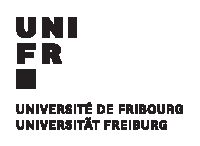
\includegraphics[width=.17\textwidth]{logos/unifr_logo}
  \hfill
    
\includegraphics[width=.4\textwidth]{logos/xi_logo}
  \vspace{30mm}
\end{figure}

{\scshape\LARGE \univname\par}\vspace{1.5cm} % University name
\textsc{\Large Bachelor Thesis}\\[0.5cm] % Thesis type
\HRule \\[0.4cm] % Horizontal line
{\huge \bfseries \ttitle\par}\vspace{0.4cm} % Thesis title
\HRule \\[1.5cm] % Horizontal line

\begin{minipage}[t]{0.4\textwidth}
\begin{flushleft} \large
\emph{Author:}\\
\href{mailto://christophe.broillet@unifr.ch}{\authorname} % Author name - remove the \href bracket to remove the link
\end{flushleft}
\end{minipage}
\begin{minipage}[t]{0.4\textwidth}
\begin{flushright} \large
\emph{Supervisors:} \\
\href{https://exascale.info/members/giuseppe-cuccu/}{\cosupname} \\ % Co-supervisor name - remove the \href bracket to remove the link
\href{https://exascale.info/phil}{\supname} % Supervisor name - remove the \href bracket to remove the link
% \\\vspace*{1ex}\emph{Co-Supervisor:} \\ % Remove these two lines if no co-supervisor is involved
% \href{https://exascale.info/members/giuseppe-cuccu/}{\cosupname} % Co-supervisor name - remove the \href bracket to remove the link
\end{flushright}
\end{minipage}\\[1cm]

February 14, 2022 % date of the official defense
\vspace*{.06\textheight}

%\large \textit{A thesis submitted in fulfillment of the requirements\\ for the degree of \degreename}\textit{ in the}\\[0.3cm] % University requirement text
\groupname\\\deptname\\ % Research group name and department name
\vfill

\footnotesize{ Boulevard de Pérolles 90 ~~$\bullet$~~ 1700~Fribourg ~~$\bullet$~~ Switzerland
            \\
            phone +41~(26)~300~84~65 ~~$\bullet$~~ \textsf{diuf-secr@unifr.ch} ~~$\bullet$~~ \textsf{www3.unifr.ch/inf}
            }


\end{center}
\end{titlepage}

% Include declaration page -- not necessary for Bachelor and Masters
% % !TEX root = ../main.tex

%----------------------------------------------------------------------------------------
% DECLARATION PAGE
%----------------------------------------------------------------------------------------

\begin{declaration}
\addchaptertocentry{\authorshipname} % Add the declaration to the table of contents
\noindent I, \authorname, declare that this thesis titled, \enquote{\ttitle} and the work presented in it are my own. I confirm that:

\begin{itemize}
\item This work was done wholly or mainly while in candidature for a research degree at this University.
\item Where any part of this thesis has previously been submitted for a degree or any other qualification at this University or any other institution, this has been clearly stated.
\item Where I have consulted the published work of others, this is always clearly attributed.
\item Where I have quoted from the work of others, the source is always given. With the exception of such quotations, this thesis is entirely my own work.
\item I have acknowledged all main sources of help.
\item Where the thesis is based on work done by myself jointly with others, I have made clear exactly what was done by others and what I have contributed myself.\\
\end{itemize}

\noindent Signed:\\
\rule[0.5em]{25em}{0.5pt} % This prints a line for the signature

\noindent Date:\\
\rule[0.5em]{25em}{0.5pt} % This prints a line to write the date
\end{declaration}

\cleardoublepage

%----------------------------------------------------------------------------------------
%	QUOTATION PAGE
%----------------------------------------------------------------------------------------
% Include only in the final submission, after the defense and all required corrections

%\vspace*{0.2\textheight}
%\noindent\enquote{\itshape Quote here}\bigbreak


%----------------------------------------------------------------------------------------
%   ABSTRACT PAGE
%----------------------------------------------------------------------------------------
\begin{abstract}
\addchaptertocentry{\abstractname} % Add the abstract to the table of contents
% !TEX root = ../main.tex

Write the thesis abstract here. Should be between half-a-page and one page of text, no newlines.

\vfill
\begin{center}
\textbf{Keywords:}~\keywordnames
\end{center}
\end{abstract}


%----------------------------------------------------------------------------------------
%	LIST OF CONTENTS/FIGURES/TABLES + TRANSITION PAGES
%----------------------------------------------------------------------------------------
\hypersetup{linkcolor=black}
\tableofcontents % Prints the main table of contents
\listoffigures % Prints the list of figures
\mainmatter % Begin numeric (1,2,3...) page numbering
\pagestyle{thesis} % Return the page headers back to the "thesis" style


%----------------------------------------------------------------------------------------
%	THESIS CONTENT - CHAPTERS
%----------------------------------------------------------------------------------------

% Include here the chapters of the thesis
% Comment/uncomment the lines to find bugs and compile faster during writing
% !TEX root = ../main.tex

\chapter{Chapter Title Here} % Main chapter title
\label{ch:name} % For referencing the chapter elsewhere, use \ref{ch:name}

%----------------------------------------------------------------------------------------

% Defining formatting commands enables consistency and separation
\newcommand{\keyword}[1]{\textbf{#1}}
\newcommand{\tabhead}[1]{\textbf{#1}}
\newcommand{\code}[1]{\texttt{#1}}
\newcommand{\file}[1]{\texttt{\bfseries#1}}
\newcommand{\option}[1]{\texttt{\itshape#1}}

%----------------------------------------------------------------------------------------

This introductory file has been edited. Please find the complete version on \url{http://www.latextemplates.com}.

Remember to keep your editor's spell checker always on. The preferred spelling is American English; using British English word spelling is accepted only if consistent throughout the thesis.

An invaluable resource when grasping for words is \url{www.thesaurus.com}. If a sentence comes more natural in another language, consider using \url{www.deepl.com} for translation as the result is typically of higher quality than Google Translate.

\section{References}

The \code{biblatex} package is used to format the bibliography and inserts references such as this one \citep{Reference1}. Use \verb|\citet| for textual citations and \verb|\citep| to wrap them in parenthesis (check the source for this text). % more here: https://en.wikibooks.org/wiki/LaTeX/More_Bibliographies#Basic_Citation_Commands
Multiple references are separated by semicolons (e.g. \citet{Reference2, Reference1}) and references with more than three authors only show the first author with \emph{et al.} indicating there are more authors (e.g. \citet{Reference3}). This is done automatically for you.

Scientific references should come \emph{before} the punctuation mark if there is one (such as a comma or period). The same goes for footnotes\footnote{Such as this footnote, here down at the bottom of the page.}.

\subsection{A Note on bibtex}

The bibtex backend used in the template by default does not correctly handle unicode character encoding (i.e. "international" characters). You may see a warning about this in the compilation log and, if your references contain unicode characters, they may not show up correctly or at all. The solution to this is to use the biber backend instead of the outdated bibtex backend. This is done by finding this command: \option{backend=bibtex} and changing it to \option{backend=biber}. You will then need to delete all auxiliary BibTeX files and navigate to the template directory in your terminal (command prompt). Once there, simply type \code{biber main} and biber will compile your bibliography. You can then compile \file{main.tex} as normal and your bibliography will be updated. An alternative is to set up your LaTeX editor to compile with biber instead of bibtex, see \href{http://tex.stackexchange.com/questions/154751/biblatex-with-biber-configuring-my-editor-to-avoid-undefined-citations/}{here} for how to do this for various editors.

\section{Tables}

Check the source for an example of the required table style.

%%%%%%%%%%%%%%%%%%%%%%%%%%%%%%%%%%%%%%%%%%%%%%%%%%%%%%%%%%%%%%%%%%%%%%%%%%%%%%%%%%
\begin{table}[h!] % positioning: here, enforced
\caption[Example]{%
  \textbf{Caption.}
  After a useful title, the caption should describe the figure by itself. A reader should know everything about this table (or figure) without having to look for its description in the text.
}
\label{tab:example}
\center
\begin{tabular}{m{25mm}lllll}
  \toprule
  & longer one & short & short & short & \textbf{bold} \\
  \midrule
  \# label 1       & {\textasciitilde{}}3034 & {\textasciitilde{}}650 & {\textasciitilde{}}650  & {\textasciitilde{}}650  & \textbf{{\textasciitilde{}}18} \\
  \# longer label & 2 & 3 & 3 & 3 & \textbf{0} \\
  \# label 3   & {\textasciitilde{}}906k & {\textasciitilde{}}436k & {\textasciitilde{}}436k & {\textasciitilde{}}436k & \textbf{{\textasciitilde{}}}\textbf{3k}\\
  \bottomrule
  \end{tabular}
\end{table}
%%%%%%%%%%%%%%%%%%%%%%%%%%%%%%%%%%%%%%%%%%%%%%%%%%%%%%%%%%%%%%%%%%%%%%%%%%%%%%%%%%

You can reference tables with \verb|Table~\ref{<label>}| where the label is defined within the table environment, see source of Table~\ref{tab:example}.

\section{Figures}

Same as Tables, check source for example. Keep all figures in the \verb|figures| folder. Strongly prefer vectorial image types (e.g.\ SVG) embedded into PDFs, over high-resolution lossless (e.g.\ PNG), over very-high-resolution lossy (e.g.\ JPG).

\begin{figure}[ht]
\centering
\decoRule\\ % avoid using these horizontal lines if you can

\includegraphics[width=0.5\textwidth]{deleteme}
\decoRule\\ % avoid using these horizontal lines if you can
\caption[Electron]{%
  \textbf{An electron.}
  Artist's impression.
}
\label{fig:electron}
\end{figure}

Sometimes figures don't always appear where you write them in the source. The placement depends on how much space there is on the page for the figure. Sometimes there is not enough room to fit a figure directly where it should go (in relation to the text) and so \LaTeX{} puts it at the top of the next page. Positioning figures is the job of \LaTeX{} and so you should only worry about making them look good!

Figures should have captions (such as in Figure~\ref{fig:electron}). The \verb|\caption| command contains two parts, the first part, inside the square brackets is the title that will appear in the \emph{List of Figures}, and so should be short. The second part in the curly brackets should contain the longer and more descriptive caption text.

The \verb|\decoRule| command is optional and simply puts an aesthetic horizontal line below the image. Avoid if possible, consider wrapping the image in a \verb|\mbox| for borders instead


\section{Typesetting mathematics}

The \enquote{Not So Short Introduction to \LaTeX} (available on \href{http://www.ctan.org/tex-archive/info/lshort/english/lshort.pdf}{CTAN}) should tell you everything you need to know for most cases of typesetting mathematics. If you need more information, a much more thorough mathematical guide is available from the AMS called, \enquote{A Short Math Guide to \LaTeX} and can be downloaded from:
\url{ftp://ftp.ams.org/pub/tex/doc/amsmath/short-math-guide.pdf}

There are many different \LaTeX{} symbols to remember, luckily you can find the most common symbols in \href{http://ctan.org/pkg/comprehensive}{The Comprehensive \LaTeX~Symbol List}.

You can write an equation, which is automatically given an equation number by \LaTeX{} like this:
\begin{verbatim}
\begin{equation}
E = mc^{2}
\label{eqn:Einstein}
\end{equation}
\end{verbatim}

This will produce Einstein's famous energy-matter equivalence equation:
\begin{equation}
E = mc^{2}
\label{eqn:Einstein}
\end{equation}

All equations you write (which are not in the middle of paragraph text) are automatically given equation numbers by \LaTeX{}. If you don't want a particular equation numbered, use the unnumbered form:
\begin{verbatim}
\[ a^{2}=4 \]
\end{verbatim}

%----------------------------------------------------------------------------------------

\section{Sectioning and Subsectioning}

You should break your thesis chapters into useful sections and subsections. \LaTeX{} automatically builds a table of Contents by looking at all the \verb|\chapter{}|, \verb|\section{}|  and \verb|\subsection{}| commands you write in the source.

%----------------------------------------------------------------------------------------

\section{In Closing}

For the final submission, generate the pdf then search it for question marks (\verb|?|). Sometimes latex misses a reference or citation and adds a question mark to fill it. Make sure to fix them all before your submission.

Good luck and have fun!

\begin{flushright}
Guide written by ---\\
Sunil Patel: \href{http://www.sunilpatel.co.uk}{www.sunilpatel.co.uk}\\
Vel: \href{http://www.LaTeXTemplates.com}{LaTeXTemplates.com}\\
\end{flushright}
 % comment this out
% % !TEX root = ../main.tex

\chapter{Introduction}
\label{ch:introduction}

Your introduction chapter here.

% \include{chapters/ ...}
% % !TEX root = ../main.tex

\chapter{Conclusion}
\label{ch:conclusions}

\section{Conclusion}
In this work we...

\section{Future Work}
The continuation of this work includes...



%----------------------------------------------------------------------------------------
%	BIBLIOGRAPHY
%----------------------------------------------------------------------------------------
\printbibliography[heading=bibintoc]


%----------------------------------------------------------------------------------------
%   APPENDIX
%----------------------------------------------------------------------------------------
% Rarely required, only if extra material particularly voluminous
% % !TEX root = ../main.tex

\chapter{Frequently Asked Questions} % Main appendix title
\label{ch:appendix}

\section{How do I change the colors of links?}

The color of links can be changed to your liking using:

{\small\verb!\hypersetup{urlcolor=red}!}, or
{\small\verb!\hypersetup{citecolor=green}!}, or
{\small\verb!\hypersetup{allcolor=blue}!}.
\noindent If you want to completely hide the links, you can use:
{\small\verb!\hypersetup{allcolors=.}!}, or even better:
{\small\verb!\hypersetup{hidelinks}!}.
\noindent If you want to have obvious links in the PDF but not the printed text, use:
{\small\verb!\hypersetup{colorlinks=false}!}.



%----------------------------------------------------------------------------------------
\end{document}
% That's all folks
